\PassOptionsToPackage{unicode=true}{hyperref} % options for packages loaded elsewhere
\PassOptionsToPackage{hyphens}{url}
%
\documentclass[]{article}
\usepackage[fontset=ubuntu]{ctex}
\usepackage[a4paper,scale=0.8]{geometry}
\usepackage{lmodern}
\usepackage{amssymb,amsmath}
\usepackage{ifxetex,ifluatex}
\usepackage{fixltx2e} % provides \textsubscript
\ifnum 0\ifxetex 1\fi\ifluatex 1\fi=0 % if pdftex
  \usepackage[T1]{fontenc}
  \usepackage[utf8]{inputenc}
  \usepackage{textcomp} % provides euro and other symbols
\else % if luatex or xelatex
  \usepackage{unicode-math}
  \defaultfontfeatures{Ligatures=TeX,Scale=MatchLowercase}
\fi
% use upquote if available, for straight quotes in verbatim environments
\IfFileExists{upquote.sty}{\usepackage{upquote}}{}
% use microtype if available
\IfFileExists{microtype.sty}{%
\usepackage[]{microtype}
\UseMicrotypeSet[protrusion]{basicmath} % disable protrusion for tt fonts
}{}
\IfFileExists{parskip.sty}{%
\usepackage{parskip}
}{% else
\setlength{\parindent}{2em}
\setlength{\parskip}{6pt plus 2pt minus 1pt}
}
\usepackage{hyperref}
\hypersetup{
            pdfborder={0 0 0},
            breaklinks=true}
\urlstyle{same}  % don't use monospace font for urls
\setlength{\emergencystretch}{3em}  % prevent overfull lines
\providecommand{\tightlist}{%
  \setlength{\itemsep}{0pt}\setlength{\parskip}{0pt}}
\setcounter{secnumdepth}{0}
% Redefines (sub)paragraphs to behave more like sections
\ifx\paragraph\undefined\else
\let\oldparagraph\paragraph
\renewcommand{\paragraph}[1]{\oldparagraph{#1}\mbox{}}
\fi
\ifx\subparagraph\undefined\else
\let\oldsubparagraph\subparagraph
\renewcommand{\subparagraph}[1]{\oldsubparagraph{#1}\mbox{}}
\fi
\usepackage{graphicx, subfigure}
\usepackage{enumerate}
\usepackage{booktabs}
\setlength{\parindent}{2em}
\pagestyle{plain}
% set default figure placement to htbp
\makeatletter
\def\fps@figure{htbp}
\makeatother
\title{第三次作业}
\author{BobAnkh}
\date{December 2020}

\begin{document}

\maketitle

\hypertarget{header-n80}{%
\subsection{1.总结人眼视网膜上的两类感光细胞的特点、作用以及它们对于视觉特征(如视觉锐度、彩色视野、眼适应性)的影响。}\label{header-n80}}
\begin{itemize}
\item
    锥状细胞。
    
    特点:数量为650-700万个,形状短粗,视色素是紫蓝质素(视黄醛+视蛋白),视蛋白不同产生吸收峰值波长在400-450nm,530-540nm,560-575nm的三种类型的锥状细胞。
    
    作用:是明视觉感受器,感受颜色。
    
    对于视觉特征的影响:中央凹的锥状细胞密度最大,在明亮时,视网膜中心部分视觉锐度最高;只有锥状细胞有色感,在同样光度照射下,不同颜色的视野范围不同;从暗转到亮视觉时,1-2分钟稳定。瞳孔3-4秒缩小,由杆状细胞(光化学反应饱和)转到锥体细胞作用。
    
\item
    杆状细胞。
    
    特点:数量为1亿-1亿3千万个,形状细长,只有亮度感,感光灵敏度是锥状细胞的100-1000倍,对红光无反应。视色素是紫红质素。
    
    作用:是暗视觉感受器,只有亮度感,对弱光敏感。
    
    对于视觉特征的的影响:杆状细胞在较暗时活动,有较高的光敏度,但不能做精细的空间分辨,且没有色感;暗适应时,瞳孔会放大,需要将褪色的紫红质素在维生素A参与下再合成,即视黄醛与视蛋白再结合,故大约30-40分钟稳定。

\end{itemize}
\hypertarget{header-n87}{%
\subsection{2.下图中的人左右眼是同色的还是异色的?试解释这一视错觉现象。}\label{header-n87}}

\centerline{
\includegraphics[scale=.5]{figures/q2.jpg}}

    通过使用“画图工具”将下图中人左右两眼的像素点抠出比较,我发现人的左右两眼实际上是同色的,但是直接看上去确实是异色的。这一视觉错觉现象是一种同时对比现象,即是刺激收到周边对比效应的影响而看到的现象。视觉系统认为左半侧有一个红色的叠加,所以在认知颜色的时候会将红色减去,因而就使得原先灰色的部分看起来像是靛青色的感觉。

\hypertarget{header-n94}{%
\subsection{3.简述视听信号编码中采用的预测编码、变换编码和熵编码的基本原理。}\label{header-n94}}

\begin{itemize}
\item
    预测编码技术:从已接收到的符号(相邻像素,如左邻、上邻、左上邻等)来预测即将接收到的符号(当前像素)最可能值;将预测值与实际值之间的差(通常接近零)进行编码,常采用线性预测函数;一个典型的代表就是差分脉冲编码调制(DPCM)。理想的预测函数通常需要知道信号的统计特性,故实际应用中,常使用更简单的线性预测函数。

\item
    变换编码技术:对图像数据做正交变换(DCT、DFT)去除图像数据中相关性,使得变换后系数在某些区域(低频区域)聚集,从而便于采用统计编码技术加以压缩(利用人的视觉分辨能力再时间空间上的限制,对于高频部分的系数进行高度压缩甚至丢弃)。

\item
    统计编码(熵编码)技术:针对图像信号幅值分布不均匀性,采用变长编码(variable length coding, VLC)以降低码率,用较短码字表示出现概率高的符号,较长码字表示出现概率低的符号,从而使得平均码长尽量逼近信息熵;针对图像中经常存在连续相同像素的情况,采用行程编码(run length coding, RLC) 等。

\end{itemize}
\hypertarget{header-n102}{%
\subsection{4.已知某线性分组码的生成矩阵为:}\label{header-n102}} 
$$
\begin{bmatrix}0 & 0 & 1 & 0 & 1 & 1 \\ 1 & 0 & 0 & 1 & 0 & 1 \\ 0 & 1 & 0 & 1 & 1 & 0 \end{bmatrix}
$$

\textbf{1) 确定该分组码的格式(n,k),并计算其校验矩阵H;}

\textbf{2) 写出该分组码可能产生的全部正确码字;}

\textbf{3) 线性分组码中,两个码字对应位上数字不同的位数称为码间距(哈明距离)。确定该分组码的最小码间距并分析其检错、纠错能力。}

\begin{enumerate}[(1)]
    \item 
        该分组码的格式为(6,3)。
        
        将G变换成典型形式$\begin{bmatrix}I\,Q \end{bmatrix}=\begin{bmatrix}1 & 0 & 0 & 1 & 0 & 1 \\ 0 & 1 & 0 & 1 & 1 & 0 \\ 0 & 0 & 1 & 0 & 1 & 1\end{bmatrix}$
        
        则可知,$Q=\begin{bmatrix}1 & 0 & 1 \\ 1 & 1 & 0 \\ 0 & 1 & 1 \end{bmatrix}$,由此得到校验矩阵$H=\begin{bmatrix}Q^T\,I \end{bmatrix}=\begin{bmatrix}1 & 1 & 0 & 1 & 0 & 0 \\ 0 & 1 & 1 & 0 & 1 & 0\\ 1 & 0 & 1 & 0 & 0 & 1 \end{bmatrix}$
        
    \item
        该分组码可能产生的全部码字为:000000,100101,010110,001011,110011,101110,011101,111000
        
    \item
        最小码距为$d_0=3$
        
        检错能力e应满足$d_0\geq e+1$,由此解得检错能力e为2
        
        纠错能力t应满足$d_0\geq 2t+1$,由此解得纠错能力t为1
\end{enumerate}

\hypertarget{header-n104}{%
\subsection{5.某16:9的LCD数字电视显示屏垂直高度为54厘米,视力为1.0的用户最远可以在离屏幕3.438米处分辨出屏幕上距离为两行高度的两根水平条纹。
}\label{header-n104}}
\textbf{1) 求该电视的显示分辨率;}

\textbf{2) 假定帧频为30Hz,亮度与色度信号按照4:1:1格式采样并10bit量化,求该数字电视系统中未经压缩的图像数据的码率(bps).}

\begin{enumerate}[(1)]
    \item
        由视力1.0知,$\theta=1.0$,从而可以计算得到屏幕上两行高度$d=\frac{\theta \times D}{3438}=0.001\,m$,由此可知屏幕上可以显示的行数为$n=\frac{0.54}{0.001/2}=1080$,继而由16:9的幅型比计算出显示的列数为$1920$,从而知道分辨率为$1920\times 1080$
        
    \item
        根据分辨率可以知道,这样的一幅图像的像素点数目为$1920\times 1080=2073600$,继而由采样格式和量化比特数可知这样一幅图像的数据量为$2073600\times \frac{4+2}{4}\times 10=31104000\,bit$,最后根据帧频可知该数字电视系统中未经压缩的图像数据码率为$31104000\times 30=9.3312\times 10^8\,bps$
        
\end{enumerate}
\hypertarget{header-n106}{%
\subsection{6.已知8个符号的信源,其符号出现的概率如下表所示:}\label{header-n106}}
$$
\begin{bmatrix}x_i\\ p_i  \end{bmatrix}=\begin{bmatrix}x_1 & x_2 & x_3 & x_4 & x_5 & x_6 & x_7 & x_8 \\ 0.4 & 0.2 & 0.15 & 0.10 & 0.06 & 0.04 & 0.03 & 0.02 \end{bmatrix}
$$

\textbf{1) 求信源的熵H;}

\textbf{2) 按照最小码方差原则,对信源进行Huffman编码,并求本次编码的编码效率和码方差;}

\textbf{3) 求符号串 $x_1 x_1 x_3 x_8 x_5 x_2 x_6$ 的算术编码数值.}

\begin{enumerate}[(1)]
    \item 
        信源的熵$H=-\sum_i p_i\log_2p_i=2.4298\,bit$
        
    \item
        按照最小码方差原则进行Huffman编码,编码如下图所示:
        
        \centerline{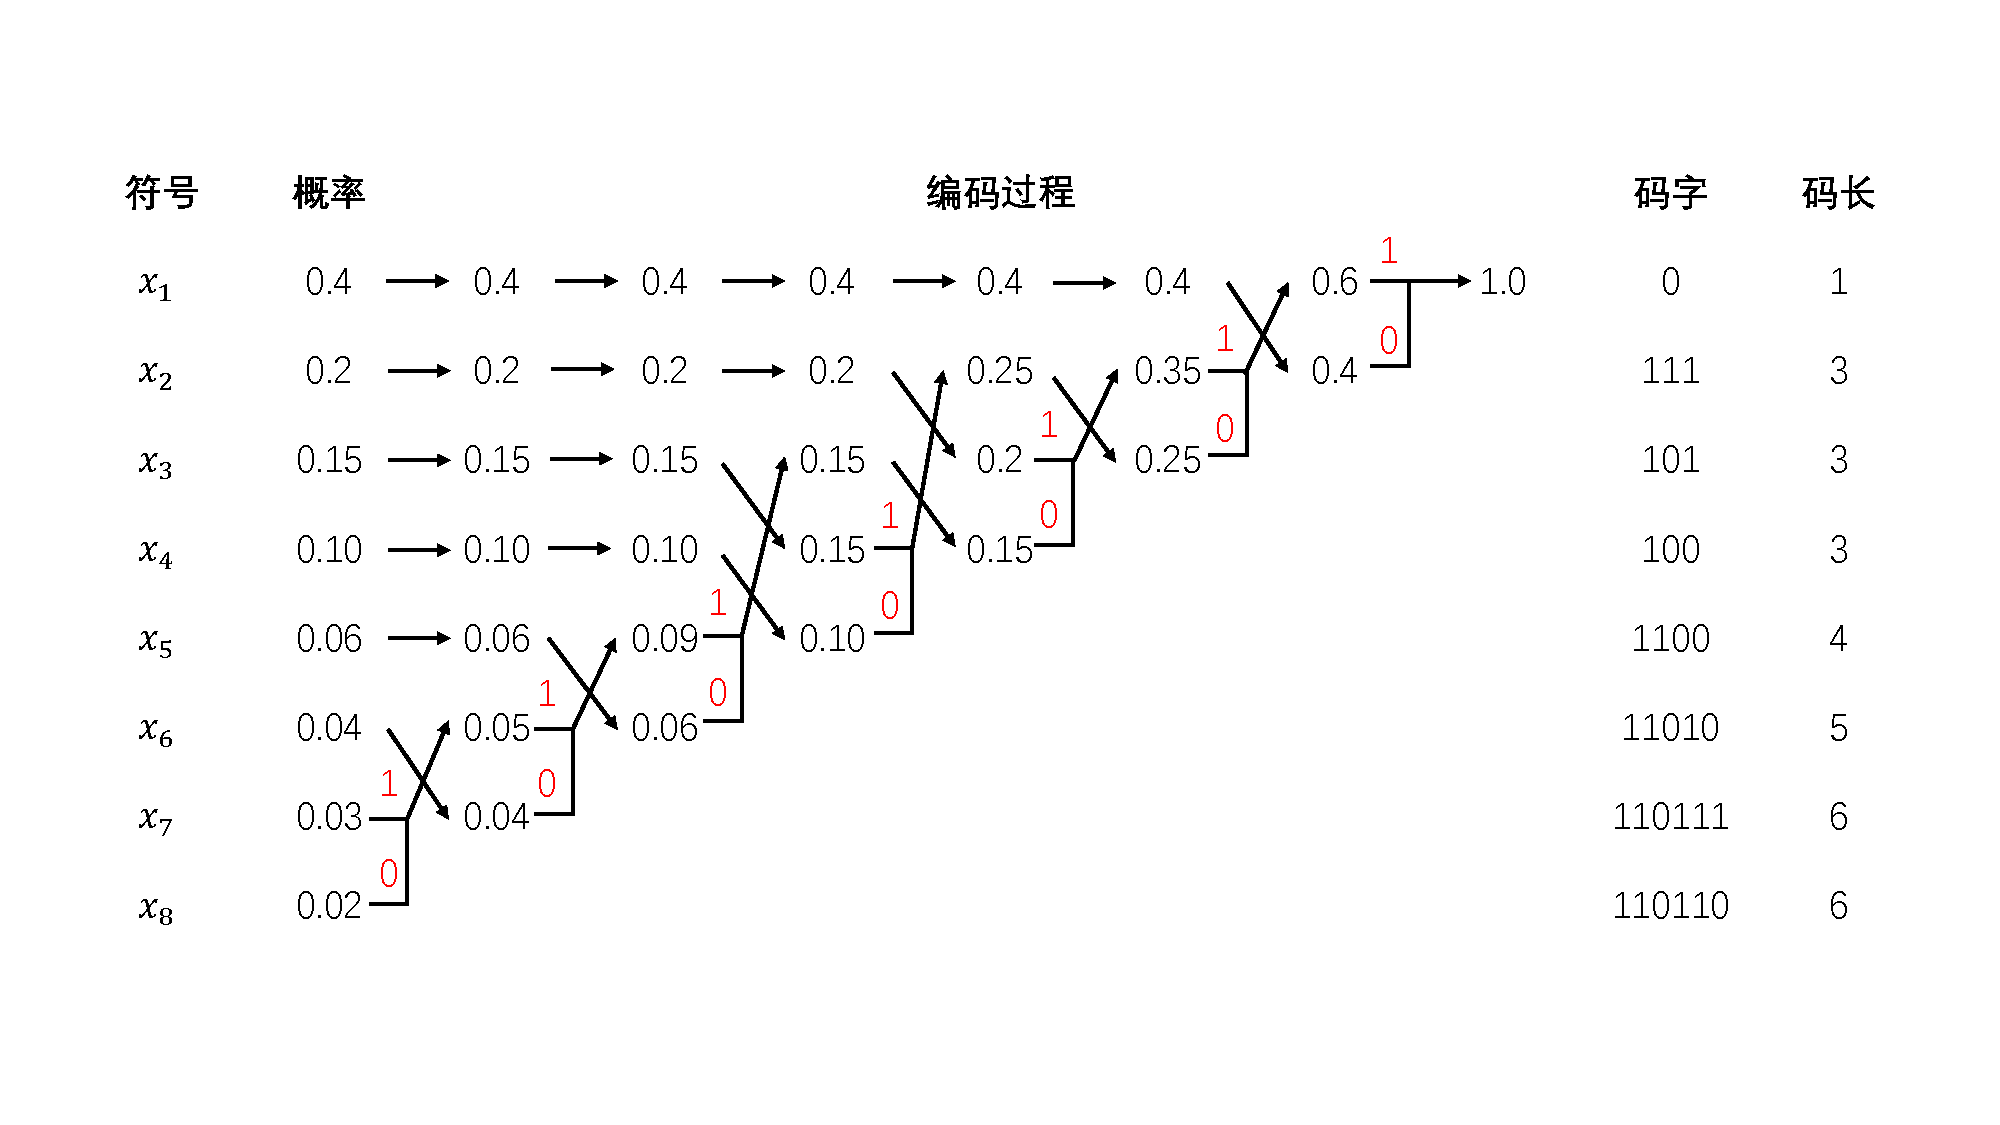
\includegraphics[width=\linewidth]{figures/encode.pdf}}
        
        根据上述编码结果可求得平均码长:$\bar{L}=\sum_{n=1}^8 p_n L_n=2.49$
        
        从而可求得编码效率$\eta=\frac{H}{\bar{L}}=97.59\,\%$
        
        码方差$\sigma^2=E((L_N-\bar{L})^2)=\sum_{n=1}^8 p_n (L_n-\bar{L})^2=2.0099$
    \item
    计算算数编码数值:
    
        \begin{table}[h]
            \centering
            \begin{tabular}{|c|c|}
                \hline
                符号 & 区间 \\
                \hline
                $x_1$ & $[0,0.4)$ \\
                \hline
                $x_1$ & $[0,0.16)$ \\
                \hline
                $x_3$ & $[0.096,0.12)$ \\
                \hline
                $x_8$ & $[0.11952,0.12)$ \\
                \hline
                $x_5$ & $[0.119928,0.1199568)$ \\
                \hline
                $x_2$ & $[0.11993952,0.11994528)$ \\
                \hline
                $x_6$ & $[0.1199447616,0.119944992)$ \\
                \hline
            \end{tabular}
        \end{table}
    
    因此其算术编码结果为$[0.1199447616,0.119944992)$中的任一数,如可取0.1199448
\end{enumerate}


\end{document}
